\chapter{La genesis del análisis de Fourier}

\epigraph{Respecto a las investigaciones de d'Alembert y Euler, ¿no podría añadirse que, si conocían esta expansión, hicieron un uso muy imperfecto de ella? Ambos estaban persuadidos de que una función arbitraria y discontinua nunca podría resolverse en series de este tipo, y ni siquiera parece que alguien hubiera desarrollado una constante en cosenos de arcos múltiples, el primer problema que tuve que resolver en la teoría del calor.}{\textit{J. Fourier}, 1808-9}

\section{Introducción histórica}

Durante el siglo XVIII, matemaáticos como Jean Le Rond d'Alembert(1717-1783) y Leonhard Euler (1707-1783) investigaron
la ecuación de onda para describir el movimiento de una cuerda vibrante \parencite{stein2003}. Aunque en 1753 Daniel
Bernulli (1700-1782) propuso que cualquier movimiento en la cuerda podía expresarse como una suma infinita de
oscilaciones sinusoidales (armónicos), Euler y d'Alembert Euler y d'Alembert rechazaron la propuesta de Bernoulli,
argumentando que una suma de funciones suaves y periódicas (como senos y cosenos) jamás podría representar una curva
que no fuera inherentemente suave o que tuviera comportamientos no periódicos en su origen
\parencite{rodriguez-zuazua}. En esa época, se creía firmemente que una función con discontinuidades nunca podría ser
representada por una serie de funciones continuas y suaves como el seno y el coseno.

La revolución en el pensamiento matemático llegó con Joseph Fourier (1768-1830) a principios del siglo XIX
\parencite{sensenbaugh2023}, \parencite{wiki-fourier}. Mientras servía como prefecto en Isère, Francia, Fourier comenzó
a experimentar con la difusión térmica, adoptando un enfoque fenomenológico: no buscacaba entender qué era el calor,
sino las leyes matemáticas que gobernaban su propagación. En su memoría de 1807, \textit{Mémoire sur la propagation de
    la chaleur dans les corps solides}, \parencite{fourier1807}, Fourier derivó la ecuación del calor basándose en el
principio de conservación de la energía y en la ley que establece que el flujo de calor es proporcional al gradiente
negativo de la temperatura.

\section{Derivación de la ecuación del calor}

Consideraremos una barra tan delgada que podemos pensar en ella efectivamente como unidimensional y colocarla a lo largo del eje $x$, es decir, sea la coordenada $x$ la que denota la posición de un punto en la barra. Imaginaremos que la temperatura en cada punto de la barra es conocida en algún tiempo inicial $t = 0$ y estaremos interesados en determinar la temperatura en tiempos futuros. Se asume que la barra está envuelta en algún tipo de aislamiento para que el calor no pueda escapar sino que deba fluir a lo largo del eje $x$. También se asume que la barra es ``homogénea'' en el sentido de que su composición física es la misma en todos los puntos. Denotaremos la temperatura en la posición $x$ y tiempo $t$ por $u(x, t)$.

Ahora bien, calor y temperatura no son lo mismo. La temperatura es una propiedad que describe el calor o frío relativo de un objeto que puede medirse (en grados en alguna escala elegida) por comparación con otro objeto (por ejemplo, un termómetro). El calor es energía. Usualmente se mide en calorías o BTU (Unidades Térmicas Británicas). La conexión es simple: elevar o bajar la temperatura de algo requiere una ganancia o pérdida de energía. Cuánta energía se necesita depende de una propiedad del objeto llamada \textit{calor específico}.

Asociada con nuestra barra homogénea hay una constante $\sigma$ (el calor específico) que depende de la sustancia de la que está hecha la barra y da una medida de la cantidad de calor necesaria para elevar la temperatura de una unidad de masa en un grado. Como es más conveniente tratar con longitudes de la barra en lugar de masas, introduciremos otra constante $\delta$, la densidad de masa de la barra. Esta representa la cantidad de masa en una unidad de longitud de la barra. Así, si la barra tiene longitud $L$, la masa total de la barra es $\delta L$. Si queremos cambiar la temperatura de una barra de longitud $L$ en $T$ grados, la energía necesaria (o perdida) es $\sigma T \delta L$.

Consideremos un punto $x$ en la barra y la pequeña sección de longitud $\Delta x$ de la barra entre $x$ y $x + \Delta x$. Más adelante, tomaremos un límite cuando $\Delta x \to 0$, así que somos libres de pensar en $\Delta x$ como tan pequeño como queramos. Comencemos pensando en él lo suficientemente pequeño para que la temperatura de la sección esté bastante bien aproximada por la temperatura de su punto medio, es decir, la temperatura en el tiempo $t$ de la sección es simplemente $u(x + \frac{\Delta x}{2}, t)$. La temperatura en un tiempo posterior $t + \Delta t$ es entonces simplemente $u(x + \frac{\Delta x}{2}, t + \Delta t)$, por lo que la diferencia de temperatura en estos dos tiempos es
\begin{equation*}
    u(x + \frac{\Delta x}{2}, t + \Delta t) - u(x + \frac{\Delta x}{2}, t).
\end{equation*}

Ahora, ¿cuánta energía (calor) se necesita para cambiar la temperatura de la pequeña sección de la barra en esta cantidad? Bueno, según la definición de calor específico, podemos escribir esta energía como:
\begin{equation}
    \sigma \left[ u(x + \frac{\Delta x}{2}, t + \Delta t) - u(x + \frac{\Delta x}{2}, t) \right] \delta \Delta x.
\end{equation}

Hay otra forma de llegar a una expresión equivalente para la cantidad de calor necesaria dada anteriormente, pensando en términos de conducción de calor. Las sustancias conducen el calor de manera diferente, por eso algunas sustancias son mejores aislantes que otras. El experimento muestra que la cantidad de calor conducido a través de un punto $x$ es proporcional a la diferencia de temperaturas a cada lado de $x$. La constante de proporcionalidad se llama conductividad térmica de la sustancia y se denotará por $k$. Los físicos llaman a esta conducción ``flujo de calor'' y se expresa matemáticamente de la siguiente manera: la cantidad de calor por unidad de tiempo que cruza el punto $x$ en la dirección positiva de $x$ está dada por
\begin{equation}
    \Phi(x, t) = -k \frac{\partial u}{\partial x}(x, t).
\end{equation}

Para entender la definición de flujo de calor puede ser útil considerar una figura. Si graficamos la temperatura $u(x, t)$ como función de $x$ para algún valor fijo de $t$, la derivada parcial $\frac{\partial u}{\partial x}(x, t)$ es simplemente la derivada regular con respecto a $x$, es decir, representa la pendiente de la línea tangente a la gráfica de $u$ en el punto $(x, u(x, t))$. En el punto etiquetado $(x_1, u(x_1, t))$, esta pendiente es negativa y la ecuación (2) nos dice entonces que una cantidad positiva de calor por unidad de tiempo fluirá más allá de $x_1$ en la dirección positiva de $x$. Esto tiene sentido, ya que está más caliente justo a la izquierda de $x_1$ que justo a la derecha. En el punto etiquetado $(x_2, u(x_2, t))$, la pendiente es positiva y la ecuación (2) nos dice que una cantidad negativa de calor por unidad de tiempo fluirá más allá de $x_2$ en la dirección positiva de $x$, en otras palabras, el calor está fluyendo más allá de $x_2$ en la dirección negativa. Esto tiene sentido, ya que está más frío justo a la izquierda de $x_1$ que justo a la derecha.

Esta figura nos ayuda a visualizar la relación entre la pendiente de la temperatura y la dirección del flujo de calor:

\begin{figure}[h]
    \centering
    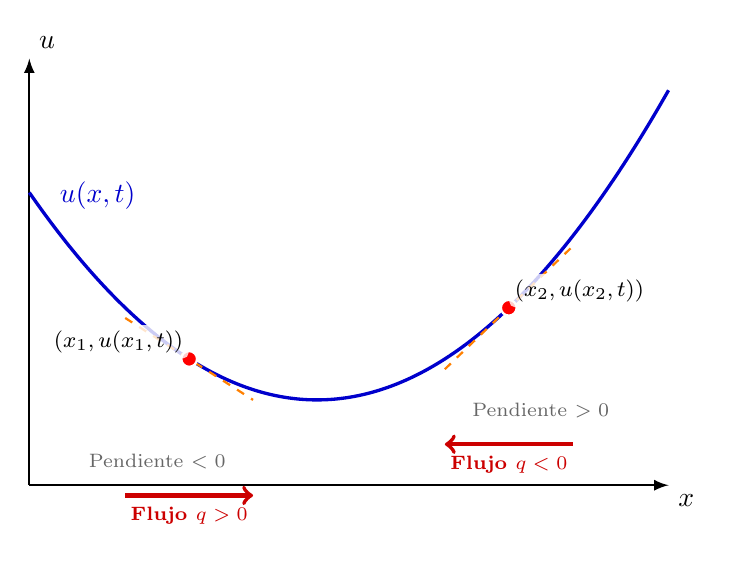
\begin{tikzpicture}
        \begin{axis}[
            width=0.8\textwidth,
            height=7cm,
            xlabel={$x$},
            ylabel={$u$},
            axis lines=middle,
            xmin=0, xmax=10,
            ymin=10, ymax=35,
            ticks=none,
            grid=none,
            domain=0:10,
            samples=100,
            clip=false,
            axis line style={-latex, thick},
            xlabel style={at={(ticklabel* cs:1)},anchor=north west, font=\bfseries},
            ylabel style={at={(ticklabel* cs:1)},anchor=south west, font=\bfseries}
        ]
            % Curve: shifted parabola u(x) = 0.6*(x-4.5)^2 + 15 (Valley)
            \addplot[blue!80!black, very thick, smooth] {0.6*(x-4.5)^2 + 15} node[pos=0.05, anchor=south west] {$u(x,t)$};

            % Parameters
            \def\xone{2.5}  % Left side (Slope < 0)
            \def\yone{17.4} 
            \def\mone{-2.4} 
            
            \def\xtwo{7.5}  % Right side (Slope > 0)
            \def\ytwo{20.4} 
            \def\mtwo{3.6}  

            % --- Point 1 (Left) Slope < 0 ---
            % Tangent
            \addplot[orange, dashed, thick, domain=1.5:3.5] {\yone + \mone*(x-\xone)};
            
            % Point
            \node[fill=red, circle, inner sep=2pt, draw=white, thick] (P1) at (axis cs:\xone, \yone) {};
            % Label with white background
            \node[above left, font=\footnotesize, fill=white, inner sep=2pt, fill opacity=0.8, text opacity=1, rounded corners=2pt] at (P1) {$(x_1, u(x_1, t))$};
            
            % Annotations
            \node[anchor=north, align=center, font=\scriptsize, color=black!60] at (axis cs:\xone-0.5, \yone-5) {{Pendiente $< 0$}};

            % Heat flow arrow (Flux > 0, flows Right)
            \draw[->, red!80!black, line width=1.5pt] (axis cs:\xone-1, \yone-8) -- (axis cs:\xone+1, \yone-8) node[midway, below, font=\bfseries\scriptsize] {Flujo $q > 0$};

            % --- Point 2 (Right) Slope > 0 ---
            % Tangent
            \addplot[orange, dashed, thick, domain=6.5:8.5] {\ytwo + \mtwo*(x-\xtwo)};
            
            % Point
            \node[fill=red, circle, inner sep=2pt, draw=white, thick] (P2) at (axis cs:\xtwo, \ytwo) {};
            % Label with white background
            \node[above right, font=\footnotesize, fill=white, inner sep=2pt, fill opacity=0.8, text opacity=1, rounded corners=2pt] at (P2) {$(x_2, u(x_2, t))$};
            
            % Annotations
            \node[anchor=north, align=center, font=\scriptsize, color=black!60] at (axis cs:\xtwo+0.5, \ytwo-5) {{Pendiente $> 0$}};

            % Heat flow arrow (Flux < 0, flows Left)
            \draw[->, red!80!black, line width=1.5pt] (axis cs:\xtwo+1, \ytwo-8) -- (axis cs:\xtwo-1, \ytwo-8) node[midway, below, font=\bfseries\scriptsize] {Flujo $q < 0$};

        \end{axis}
    \end{tikzpicture}
    \caption{Relación entre el gradiente de temperatura y el flujo de calor. Cuando la pendiente es positiva (izquierda), el calor fluye en dirección negativa. Cuando la pendiente es negativa (derecha), el calor fluye en dirección positiva.}
    \label{fig:heat_flow}
\end{figure}

Ahora volvamos a nuestra pequeña subsección de la barra entre $x$ y $x + \Delta x$. La cantidad total de calor que fluye hacia la sección de la barra por unidad de tiempo es simplemente el flujo de calor en $x$ menos el flujo de calor en $x + \Delta x$ (el signo menos aquí es debido a la dirección: en $x + \Delta x$, ``hacia la sección'' está en la dirección negativa de $x$), o sea, $\Phi(x, t) - \Phi(x + \Delta x, t)$. Durante un pequeño intervalo de tiempo entre $t$ y $t + \Delta t$, la energía total que entra en la pequeña sección de la barra es entonces
\begin{equation}
    \left[ \Phi(x, t) - \Phi(x + \Delta x, t) \right] \Delta t = k \left[ \frac{\partial u}{\partial x}(x + \Delta x, t) - \frac{\partial u}{\partial x}(x, t) \right] \Delta t.
\end{equation}

Igualando (1) y el lado derecho de (3) obtenemos
\begin{equation*}
    \sigma \left[ u(x + \frac{\Delta x}{2}, t + \Delta t) - u(x + \frac{\Delta x}{2}, t) \right] \delta \Delta x = k \left[ \frac{\partial u}{\partial x}(x + \Delta x, t) - \frac{\partial u}{\partial x}(x, t) \right] \Delta t
\end{equation*}
o bien,
\begin{equation}
    \frac{u(x + \frac{\Delta x}{2}, t + \Delta t) - u(x + \frac{\Delta x}{2}, t)}{\Delta t} = \kappa \frac{\frac{\partial u}{\partial x}(x + \Delta x, t) - \frac{\partial u}{\partial x}(x, t)}{\Delta x}
\end{equation}
donde $\kappa \equiv \frac{k}{\sigma \delta}$. Si ahora tomamos el límite de ambos lados de (4) cuando $\Delta x \to 0$, obtenemos:
\begin{equation*}
    \frac{u(x, t + \Delta t) - u(x, t)}{\Delta t} = \kappa \frac{\partial^2 u}{\partial x^2}(x, t).
\end{equation*}

Tomando el límite de esta última ecuación cuando $\Delta t \to 0$ nos da lo que se conoce comúnmente como la ecuación del calor (o difusión) unidimensional:
\begin{equation}
    \frac{\partial u}{\partial t}(x, t) = \kappa \frac{\partial^2 u}{\partial x^2}(x, t).
\end{equation}